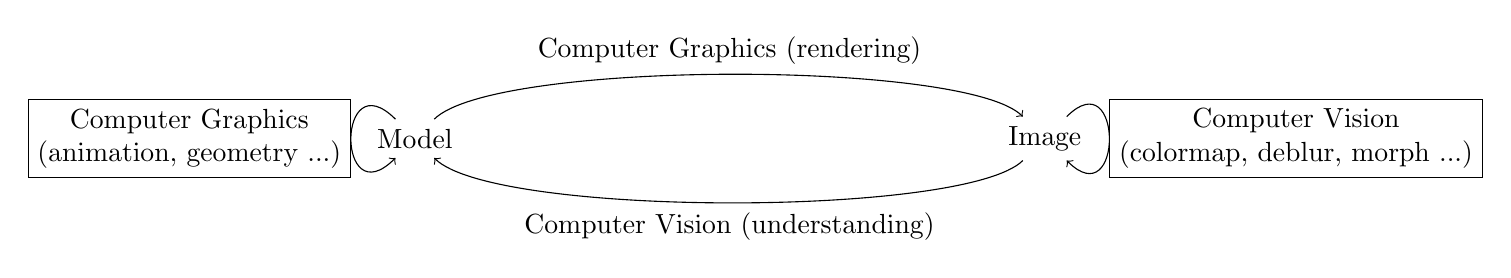
\begin{tikzpicture}[->]
    \node (A) at (0, 0) {Model};
    \node (B) at (8, 0) {Image};
    \draw[->] (A) .. controls (1, 1)
    and (7, 1) .. node[above]{Computer Graphics (rendering)} (B);
    \draw[->] (B) .. controls (7, -1)
    and (1, -1) ..  node[below]{Computer Vision (understanding)} (A);
    \draw[->] (A) .. controls (-1, 1)
    and (-1, -1) ..  node[draw, left, align=center]{Computer Graphics \\ 
    (animation, geometry ...)} (A);
    \draw[->] (B) .. controls (9, 1)
    and (9, -1) ..  node[draw, right, align=center]{Computer Vision \\ 
    (colormap, deblur, morph ...)} (B);
\end{tikzpicture}